\documentclass[11pt,letterpaper]{article}
\usepackage[utf8]{inputenc}
\usepackage{amsmath,amssymb,fullpage,graphicx}
\usepackage{subfigure}
\let\hat\widehat
\let\tilde\widetilde

\begin{document}
\subsection*{Q5-a}

\begin{verbatim}
norm_sp <- rnorm(n=25)
base_value <- seq(-3, 3, 0.01)
density_value <- dnorm(base_value)

hist(norm_sp, xlim=c(-3, 3), probability=T, xlab='X', ylab='Density',
     main='Histogram of Normal Sample')
lines(base_value, density_value, lty=3, lwd=2)

qqnorm(norm_sp)
abline(a=0, b=1, lty=3)
\end{verbatim}

\hspace*{-0.5 in} 
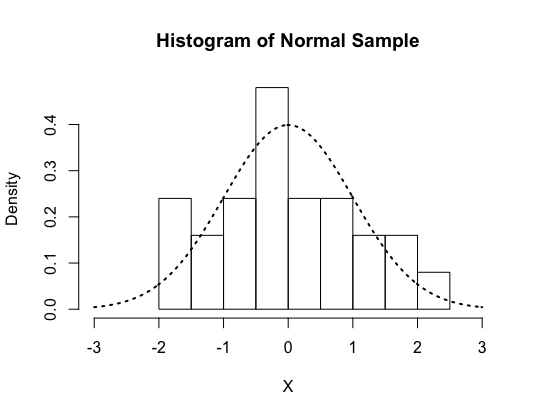
\includegraphics[scale=0.5]{q5-a.png}
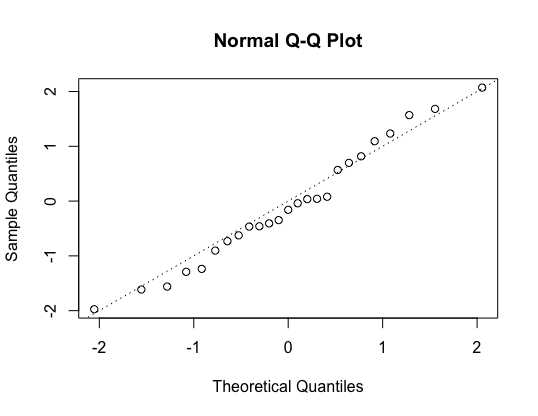
\includegraphics[scale=0.5]{q5-a-2.png}

\noindent Since all sample data are from $Normal(0,1)$, the qqplot of sample quantile fits theoretically normal quantile very well. Also, we can perceive that the standard normal curve fits the histogram anywhere, thus the sample data distributed approximately normal. 

\newpage
\subsection*{Q5-b}
\begin{verbatim}
Z <- rnorm(n=25)
U <- runif(n=25)
Y <- Z/U
base_value <- seq(-8, 8, 0.01) 
density_value <- dnorm(base_value)

hist(Y, probability=T, xlim=c(-8, 8), ylim=c(0, 0.4))
lines(base_value, density_value, lty=3, lwd=2)

qqnorm(Y)
abline(a=0, b=1, lty=3)
\end{verbatim}

\hspace*{-1 in} 
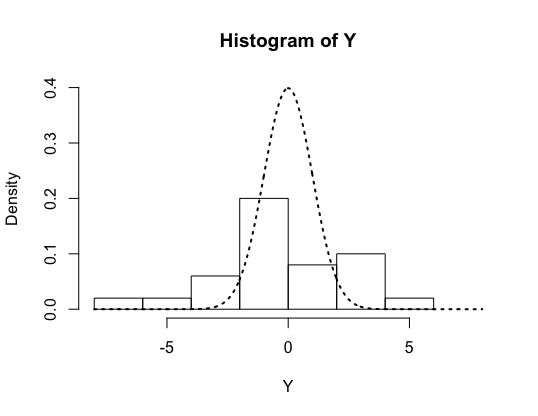
\includegraphics[width=100mm]{q5-b-1.png}
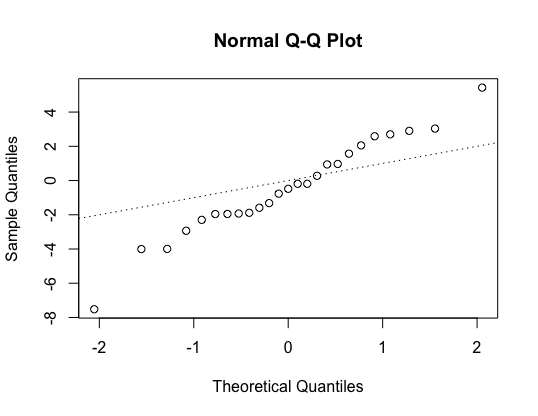
\includegraphics[width=100mm]{q5-b-2.png}

\noindent In this case, Y doesn't seem to follow standard normal distribution. From the histogram, we can perceive that sample values from Y are smaller in low quantiles (sample data is denser at left tail than standard normal), and larger at upper quantiles (denser at right tail than standard normal). In qqplot, first half of sample quantiles are smaller than standard normal quantiles, while second half of those are larger than theoretical quantiles. 


\end{document}